\documentclass[10pt,a4paper]{amsart}
\usepackage[margin=19mm]{geometry}
\usepackage{amsmath,amssymb,mathtools}
\usepackage[scr=rsfs,cal=euler]{mathalfa}
\usepackage{xfrac}
\usepackage[unicode,hidelinks,bookmarks=false]{hyperref}
\newcommand{\ie}{i.e.\ }
\newcommand{\cf}{cf.\ }
\newcommand{\resp}{respectively\ }
\newcommand{\Subsection}{\subsection}
\providecommand{\nobreakdash}{\nobreak\hbox{-}}
\setlength{\emergencystretch}{2em}
\multlinegap0pt
\usepackage{tikz}
\usepackage{amssymb}
\usepackage{xcolor}
\usepackage{csquotes}
\usepackage{mathtools}
\newtheorem{lemma}{Lemma}
\def\graph{\mathcal{G}}
\newcommand{\set}[1]{\{#1 \}}
\title{Transitive Extensions of Automorphism Groups of Generic Structures}
\author{Felipe Estrada}
\date{Source: arXiv:2604.12146v1 (CC BY 4.0)}
\begin{document}
\maketitle

\noindent\emph{Source and licence.} Transitive Extensions of Automorphism Groups of Generic Structures. Version arXiv:2604.12146v1 (CC BY 4.0), distributed by arXiv under the Creative Commons Attribution 4.0 International licence, http://creativecommons.org/licenses/by/4.0/, as recorded in the arXiv licence metadata for this exact version and shown on the abstract page https://arxiv.org/abs/2604.12146v1. Full licence notice: \texttt{licenses/arxiv-2604.12146-CC-BY-4.0.txt}.\par\smallskip

\noindent\textit{Editorial scope.} Counted unit: the article's lemma palettes (source0.tex lines 387--396). The article's complete original proof of it is delivered with it (source0.tex lines 397--464, one \texttt{proof} environment of 68 lines). No mathematics is written, repaired or re-derived: the statement and the proof are the article's own lines, in the article's own notation, and no retained line is substituted or re-flowed.  Retained uncounted as the source-local context the proof needs: lines 373--375.  Nothing was omitted from any retained span, so the package carries no omission record.  No retained line contains a citation, so the wrapper carries no bibliography and no bibliography entry.  The retained lines contain the article's own diagram code, which the wrapper typesets with the standard tikz packages; no image file is delivered and the package declares no asset dependency.  Editorial formatting only, in addition: an AMS \texttt{amsart} preamble that restates the article's own declarations and macros used by the retained lines, namely the environments \texttt{lemma} on separate counters, together with the standard packages those lines need.  The retained environments print in this document as Lemma 1 in order of appearance, whereas the article prints the same items with the numbering of its own full document.  The complete native source of the article as distributed in the arXiv e-print for this exact version is bundled unchanged as \texttt{sources/198387/source0.tex}.
\begin{lemma}\label{Conditions for generic Graph extensions}
    Let $\graph = (G, R_1, \dots, R_n)$ be an ultrahomogeneous edge-colored $k$-hypergraph in $n$ colors. If $\graph$ has a transitive one-point extension $\graph'$ in canonical form, then $\graph'$ is an edge-colored $(k+1)$-hypergraph $(G, R'_1, \dots, R'_n)$ with $n$ colors and no additional structure.
\end{lemma}

\begin{lemma}\label{existence of palettes}
    Let $\graph$ be the generic edge-colored graph with $n$ colors. If $\graph$ has a transitive one-point extension $\graph'$, then there exists a set $A \subseteq M_n^4$ of 4-multisets such that
    \begin{enumerate}
        \item Every 3-multiset in $M_n^3$ is contained in a unique multiset in $A$.

        \item All multisets of the form $\set{i, i, j, j}$ are in $A$ (Including when $i = j$).

        \item If $\set{i, i', j, j'} \in A$ and $\set{i, i', k, k'} \in A$, then $\set{j, j', k, k'}, \in A$
    \end{enumerate}
\end{lemma}

\begin{proof}
    We shall construct the set $A$ starting from a transitive extension $\graph'$ of $\graph$.

    By Lemma \ref{Conditions for generic Graph extensions}, $(G')^3\setminus \Delta_{G '}^3$ can be colored as $n$ disjoint hypergraphs, $R_1', \dots, R_n'$, which correspond to the edge colors $R_1, \dots, R_n$ of $\graph$ by the rule
    $$R_i(x,y) \Longleftrightarrow R_i'(x,y, 0).$$
    Now, given a triples of elements $(a,b,c)$ in ${G}$, their setwise orbit in $\graph$ is completely determined by the distribution of colors of the triangle they form. i.e. whether $\set{a,b,c}$ maps to $\set{a', b', c'}$ as a set depends only on whether the number of edges of each color is the same for both of them. In $\graph'$ this same setwise orbit is instead determined by which color the hyperedge between them is. Thus, the latter must be determined from the former. That is, there exists a function
    $$f : M_n^3 \rightarrow \set{1, \dots,n}$$
    which maps the multiset of colors on a triangle to the color of the corresponding hyperedge. Another way to think of the input of $f$ is not as the colors of the triangle formed by a triple $\{a,b,c\}$ in $\graph$, but rather as the colors of the hyperedges $\{a, b, 0\}$, $\{a, c, 0\}$ and $\{b, c, 0\}$ in $\graph'$. That is, if given the color of the hyperedge relations on triples from $\set{0, a,b,c}$ which include $0$, the color of $\{a,b,c\}$ is determined. But this can be expressed as a sentence in the type of $0$, so by transitivity this must be true if we replace $0$ for any other element. That is, given four arbitrary points such that colors of three of their hyperedges form a multiset $\set{i, j, k}$, the fourth hyperedge must have color $f(\set{i, j, k})$. Define now an additional function $\hat{f}: M_n^3 \rightarrow M_n^4$ by
    $$\hat{f}(\set{i,j,k}) = \set{i, j, k, {f}(\set{i,j,k})}.$$
    We define $A$ as the image of this function. Or equivalently as the set of multisets of colors which arise as the hyperedge colors of the four sub-triples of any 4-tuple in $\graph'$. We prove that $A$ satisfies the properties in the statement:
    \begin{enumerate}
        \item Any multiset $t \in M_n^3$ is, by construction, contained in $\hat f(t) \in A$. If there was another such multiset, there would would be two 3-tuples $(a,b,c)$ and $(a', b', c')$, such that the multiset of colors of the triangle they form in $\graph$ is $t$, but the hyperedges between them in $\graph'$ have different colors, meaning they are in the same $\graph$-orbit but not $\graph'$ orbit, which is a contradiction.

        \item Suppose $\{i, i, j, j\} \not \in A$ , then $f(\{i, i, j\})$ is some $k \neq j$. That is $\set{i,i,j,k} \in A$. Consider the following subgraph of $\graph$ whose edges are colored with colors $i, j, k$:

        \begin{center}
        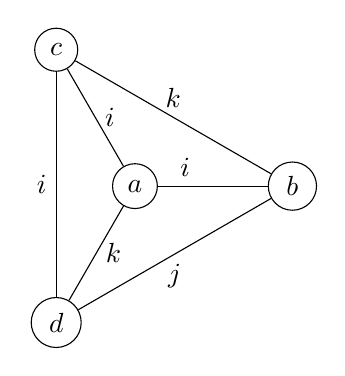
\begin{tikzpicture}
        

        \node[circle, draw] (a) at (0: 0) {$a$};
        \node[circle, draw] (b) at (0: 2) {$b$};
        \node[circle, draw] (c) at (120: 2) {$c$};
        \node[circle, draw] (d) at (240: 2) {$d$};

        \draw (a) -- node[midway, above, xshift=-10pt] {$i$} (b);
        \draw (a) -- node[midway, right] {$i$} (c);
        \draw (a) -- node[midway, right] {$k$} (d);
        \draw (b) -- node[midway, above] {$k$} (c);
        \draw (b) -- node[midway, below] {$j$} (d);
        \draw (c) -- node[midway, left] {$i$} (d);
            
        \end{tikzpicture}
        \end{center}

        Notice that for every triangle, its multiset of colors is a sub-multiset of $\set{i,i,j,k}$, so $\set{a,b,d}$ and $\set{b,c, d}$ have color $i$ while $\set{a,b,c}$ and $\set{a,c, d}$ have color $j$, therefore the triples from $\{a, b, c, d\}$ have colors $\{i, i, j, j\}$, and so this multiset is in $A$, contradicting the assumption.

        \item Suppose $\set{i, i', j, j'}$ and $\set{i, i', k, k'}$ are both in $A$. Consider the following subgraph of $\graph$ whose edges are colored with colors $i, i', j, k$

        \begin{center}
        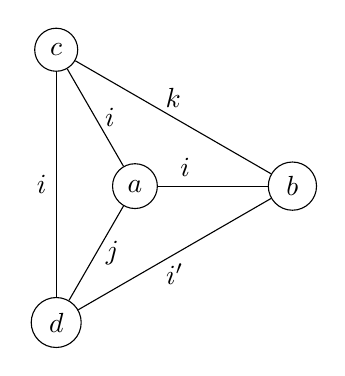
\begin{tikzpicture}
        

        \node[circle, draw] (a) at (0: 0) {$a$};
        \node[circle, draw] (b) at (0: 2) {$b$};
        \node[circle, draw] (c) at (120: 2) {$c$};
        \node[circle, draw] (d) at (240: 2) {$d$};

        \draw (a) -- node[midway, above, xshift=-10pt] {$i$} (b);
        \draw (a) -- node[midway, right] {$i$} (c);
        \draw (a) -- node[midway, right] {$j$} (d);
        \draw (b) -- node[midway, above] {$k$} (c);
        \draw (b) -- node[midway, below] {$i'$} (d);
        \draw (c) -- node[midway, left] {$i$} (d);
            
        \end{tikzpicture}
        \end{center}

        Notice the following:
        \begin{itemize}
            \item The edges in $\{a,b,c\}$ are colored $\{i, i , k\} \subseteq \{i, i, k, k\} \in A$ (by (2)), so $\{a,b,c\}$ has color $k$.
            \item The edges in $\{a,b,d\}$ are colored $\{i, i', j\} \subseteq \{i, i', j, j'\} \in A$, so $\{a,b,c\}$ has color $j'$.
            \item The edges in $\{a,c,d\}$ are colored $\{i, i , j\} \subseteq \{i, i, j, j\} \in A$ (by (2)), so $\{a,b,c\}$ has color $j$.
            \item The edges in $\{b,c,d\}$ are colored $\{i, i' , k\} \subseteq \{i, i', k, k'\} \in A$, so $\{a,b,c\}$ has color $k'$.
        \end{itemize}
        Thus, the triples from $\{a, b, c, d\}$ have colors $\{j, j', k, k'\}$, and so this multiset is in $A$, as desired.
    \end{enumerate}
    Thus, $A = \textrm{Im}(\hat f)$ satisfies the conditions in the statement.
\end{proof}

\end{document}
